% !TeX spellcheck = en_US
% !TeX spellcheck = ru_RU

\documentclass[a4paper, 12pt]{article}

\usepackage[english, russian]{babel}
\usepackage[utf8]{inputenc}
\usepackage[T2A]{fontenc}

\usepackage{hyperref}
\hypersetup{
  linkcolor=blue,
  urlcolor=cyan,
  colorlinks=true
}

\usepackage{graphicx}
\usepackage{float}


\title{НЕКРОНОМИКОН\\или ещё одна книга о Raspberry Pi 2B+\\(для чайников)}
\author{Михаил Ферапонтов | Алексей Савчук | Вадим Яровой}
\date{\the\year}

\begin{document}

\maketitle

\newpage
\begin{figure}[H]
  \centering
  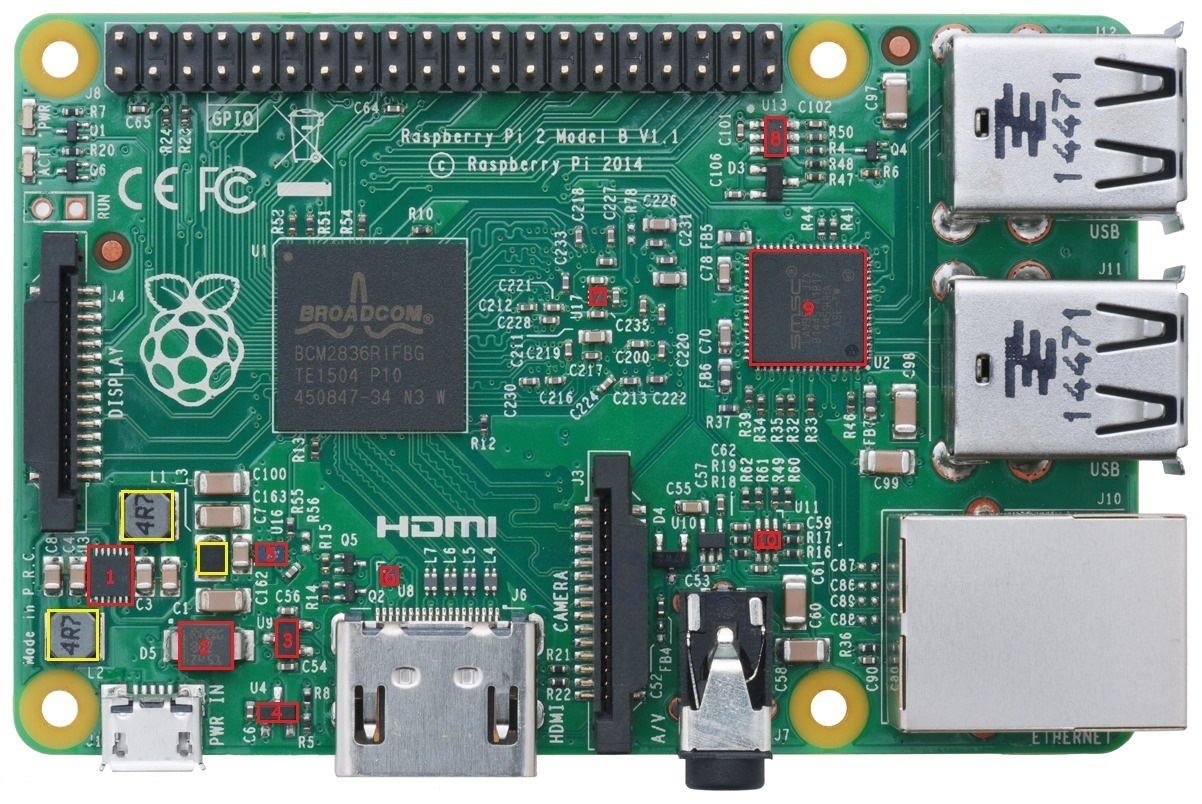
\includegraphics[width=\textwidth]{img/raspberry-photo-edited.jpg}
\end{figure}

\newpage
1. [U3 | PAM2306AYPKE] DUAL HIGH-EFFICIENCY PWM STEP-DOWN DC-DC CONVERTER
\begin{figure}[H]
  \centering
  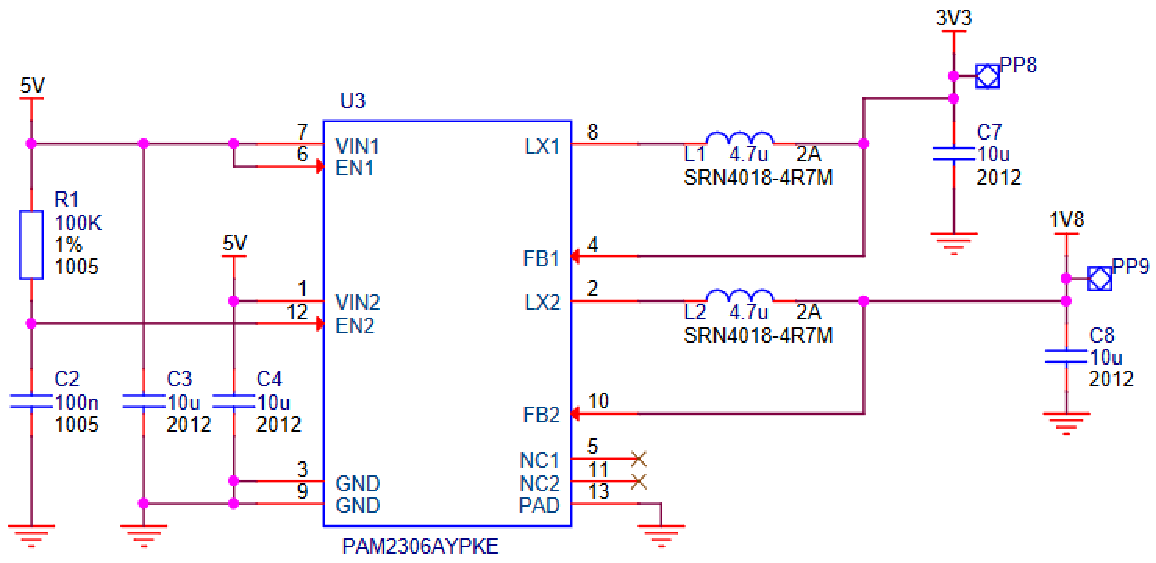
\includegraphics[width=\textwidth]{img/U3.pdf}
\end{figure}

\newpage
2. [D5 | SMBJ5.0A] Диод в схеме с идеальным диодом (этот на обратной стороне)
\begin{figure}[H]
  \centering
  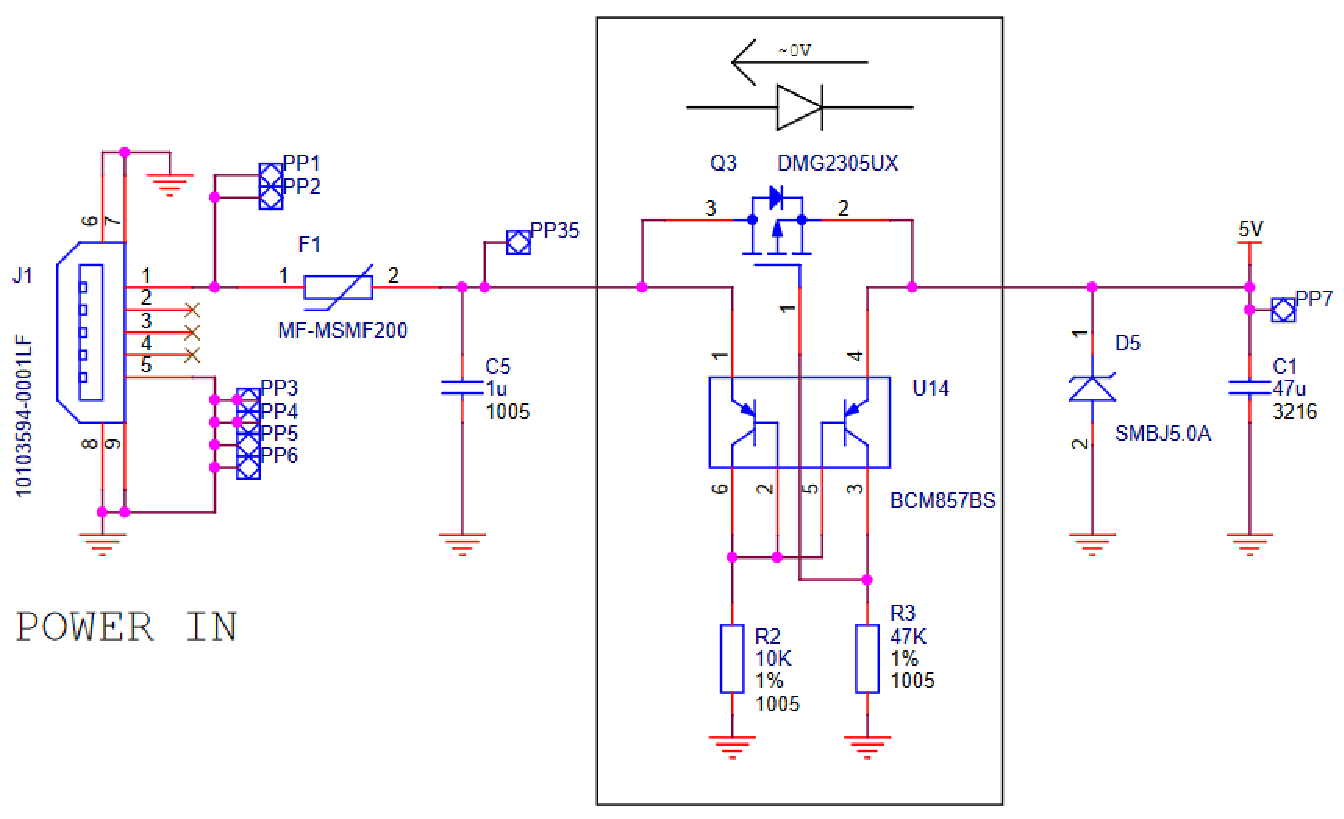
\includegraphics[width=\textwidth]{img/D5.pdf}
\end{figure}

\newpage
4. [U4 | APX803-46SAG]
\begin{figure}[H]
  \centering
  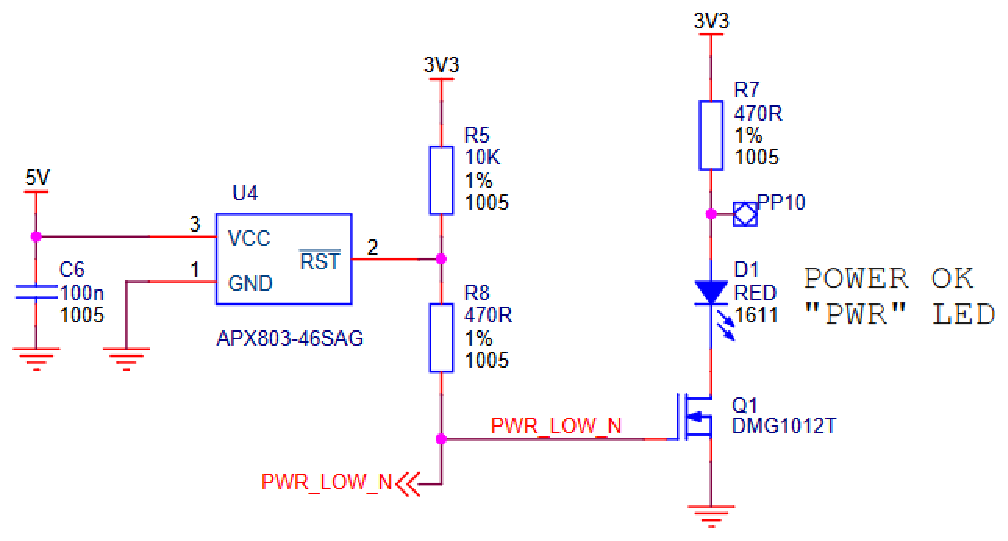
\includegraphics[width=\textwidth]{img/U4.pdf}
\end{figure}

\newpage
5. [U16 | NCP6343]
\begin{figure}[H]
  \centering
  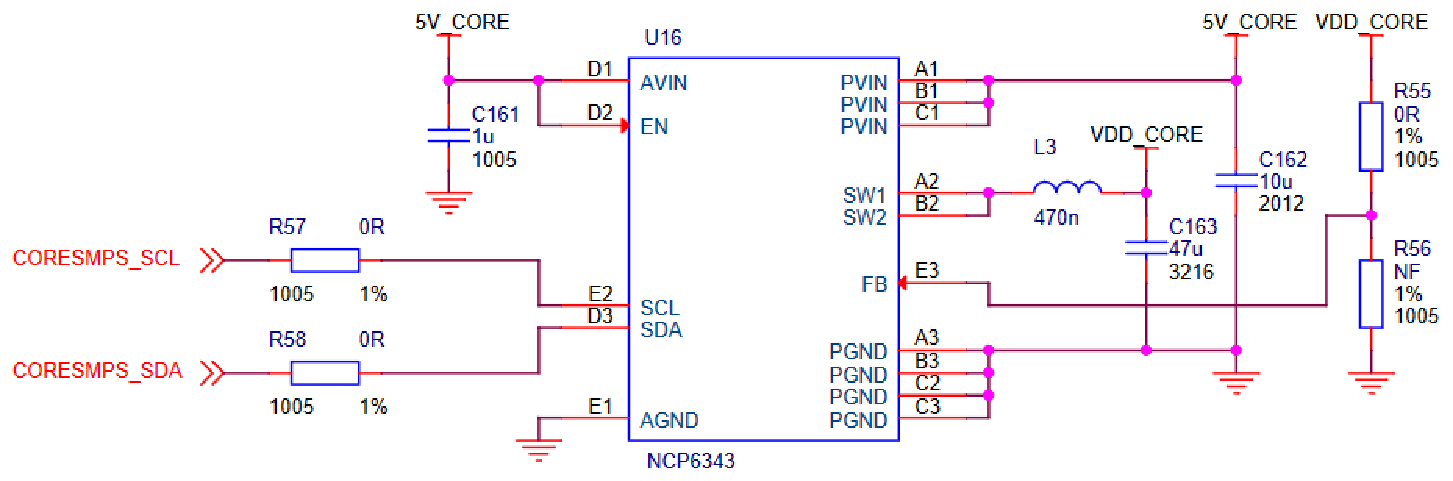
\includegraphics[width=\textwidth]{img/U16.pdf}
\end{figure}

\newpage
10. [U11 | NC7WZ16]
\begin{figure}[H]
  \centering
  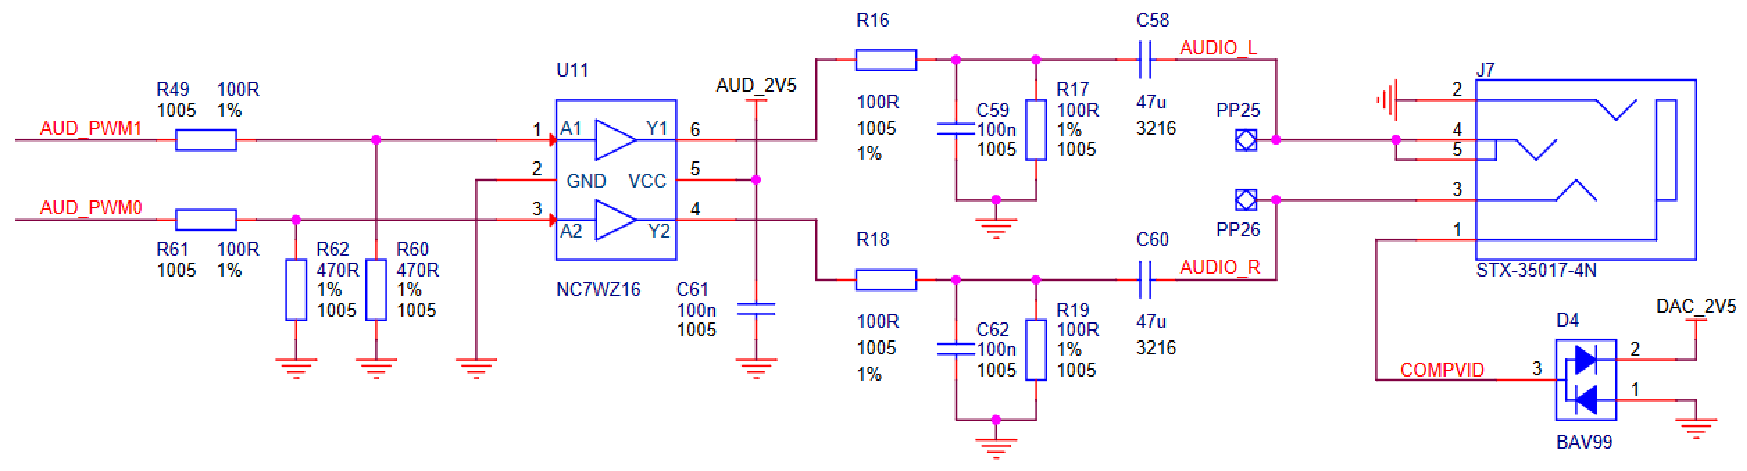
\includegraphics[width=\textwidth]{img/U11.pdf}
\end{figure}



% ---------------------------
% Ниже будет инфа про драйвер
% ---------------------------

\newpage
0. [изображение драйвера]
\begin{figure}[H]
  \centering
  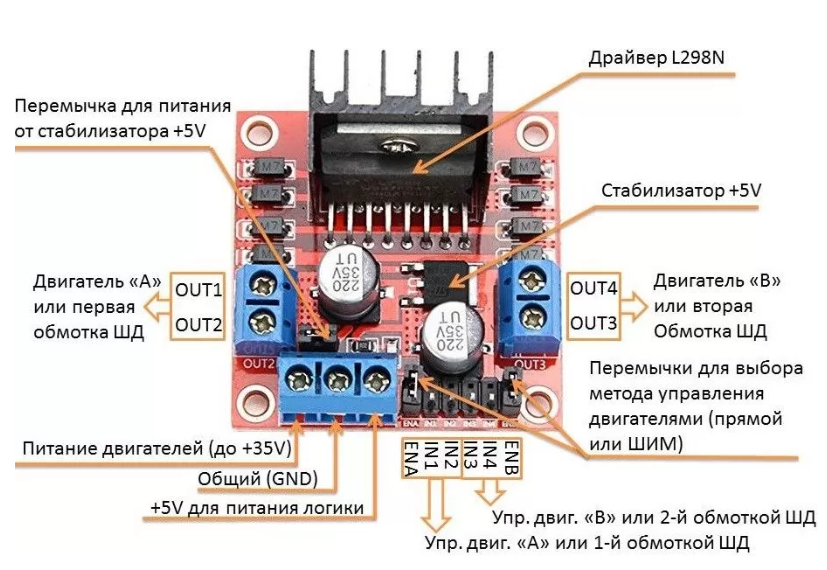
\includegraphics[width=\textwidth]{img/L298N/L298N_simple.png}
\end{figure}

\newpage
0-1. [пронумерованные компоненты]
\begin{figure}[H]
  \centering
  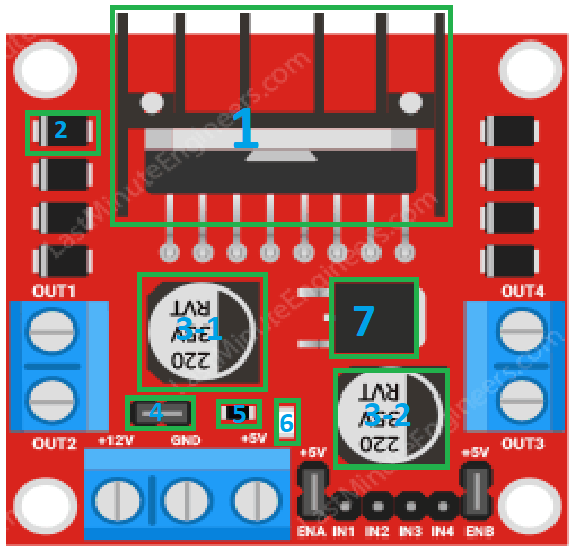
\includegraphics[width=\textwidth]{img/L298N/L298N_numbers.png}
\end{figure}

\newpage
1. [Драйвер L298N]
\begin{figure}[H]
  \centering
\end{figure}

\newpage
2. [M7]
\begin{figure}[H]
  \centering
\end{figure}

\newpage
3. [220 35v UT]
\begin{figure}[H]
  \centering
\end{figure}

\newpage
4. [перемычка для питания от стабилизатора 5v]
\begin{figure}[H]
  \centering
\end{figure}

\newpage
5. [??]
\begin{figure}[H]
  \centering
\end{figure}

\newpage
6. [??]
\begin{figure}[H]
  \centering
\end{figure}

\newpage
7. [стабилизатор 5V]
\begin{figure}[H]
  \centering
\end{figure}

\end{document}
